\documentclass[12pt,a4paper,bibliography=totocnumbered,listof=totocnumbered]{scrartcl}
\usepackage[ngerman]{babel}
\usepackage[utf8]{inputenc}
\usepackage{amsmath}
\usepackage{amsfonts}
\usepackage{amssymb}
\usepackage{csquotes}
\usepackage{graphicx}
\usepackage{fancyhdr}
\usepackage{float}
\usepackage{tabularx}
\usepackage{geometry}
\usepackage{setspace}
\usepackage[right]{eurosym}
\usepackage[printonlyused]{acronym}
%\usepackage{subfig}
\usepackage{floatflt}
\usepackage[usenames,dvipsnames]{color}
\usepackage{colortbl}
\usepackage{paralist}
\usepackage{array}
\usepackage{subcaption}
\usepackage{wrapfig}
\usepackage{titlesec}
\usepackage{parskip}
\usepackage[right]{eurosym}
\usepackage{picins}
\usepackage[subfigure,titles]{tocloft}
\usepackage[pdfpagelabels=true]{hyperref}
\usepackage[export]{adjustbox}

\usepackage{listings}
\lstset{basicstyle=\footnotesize, captionpos=b, breaklines=true, showstringspaces=false, tabsize=2, frame=lines, numbers=left, numberstyle=\tiny, xleftmargin=2em, framexleftmargin=2em}
\makeatletter
\def\l@lstlisting#1#2{\@dottedtocline{1}{0em}{1em}{\hspace{1,5em} Lst. #1}{#2}}
\makeatother

\geometry{a4paper, top=27mm, left=30mm, right=20mm, bottom=35mm, headsep=10mm, footskip=12mm}

\hypersetup{unicode=false, pdftoolbar=true, pdfmenubar=true, pdffitwindow=false, pdfstartview={FitH},
	pdftitle={Learning Diary},
	pdfauthor={Christian Neubauer },
	pdfsubject={Independent Coursework},
	pdfcreator={\LaTeX\ with package \flqq hyperref\frqq},
	pdfproducer={pdfTeX \the\pdftexversion.\pdftexrevision},
	pdfkeywords={Abschlussarbeit},
	pdfnewwindow=true,
	colorlinks=true,linkcolor=black,citecolor=black,filecolor=magenta,urlcolor=black}
\pdfinfo{/CreationDate (D:20110620133321)}

\begin{document}

\titlespacing{\section}{0pt}{12pt plus 4pt minus 2pt}{-6pt plus 2pt minus 2pt}

% Kopf- und Fusszeile
\renewcommand{\sectionmark}[1]{\markright{#1}}
\renewcommand{\leftmark}{\rightmark}
\pagestyle{fancy}
\lhead{}
\chead{}
\rhead{\thesection\space\contentsname}
\lfoot{Independent Coursework}
\cfoot{}
\rfoot{\ \linebreak Seite \thepage}
\renewcommand{\headrulewidth}{0.4pt}
\renewcommand{\footrulewidth}{0.4pt}

% Vorspann
\renewcommand{\thesection}{\Roman{section}}
\renewcommand{\theHsection}{\Roman{section}}
\pagenumbering{Roman}

% ----------------------------------------------------------------------------------------------------------
% Titelseite
% ----------------------------------------------------------------------------------------------------------
\thispagestyle{empty}
\begin{center}
	
\includegraphics[scale=1]{Bilder/HTW_Logo_rgb.png}\\
	\vspace*{2cm}
	\Large
	\textbf{Fachbereich 4}\\
	\textbf{Informatik, Kommunikation und Wirtschaft}\\
	\vspace*{2cm}
	\Huge
	\textbf{Independent Coursework I}\\
	\vspace*{0.5cm}
	\large
	\vspace*{1cm}
	\textbf{Umsetzung einer iOS Applikation basierend auf dem Masterprojekt Neeedo.com mit Swift }\\
	\vspace*{2cm}
	
	\vfill
	\normalsize
	\newcolumntype{x}[1]{>{\raggedleft\arraybackslash\hspace{0pt}}p{#1}}
	\begin{tabular}{x{6cm}p{7.5cm}}
		\rule{0mm}{5ex}\textbf{Autor:} & Christian Neubauer\newline Matr.Nr. 547617 \\ 
		\rule{0mm}{5ex}\textbf{Prüfer:} & Prof. Dr. Jung \\ 
		\rule{0mm}{5ex}\textbf{Abgabedatum:} & 24.03.2016 \\ 
	\end{tabular} 
\end{center}
\pagebreak

% ----------------------------------------------------------------------------------------------------------
% Verzeichnisse
% ----------------------------------------------------------------------------------------------------------
% TODO Typ vor Nummer
\renewcommand{\cfttabpresnum}{Tab. }
\renewcommand{\cftfigpresnum}{Abb. }
\settowidth{\cfttabnumwidth}{Abb. 10\quad}
\settowidth{\cftfignumwidth}{Abb. 10\quad}

\titlespacing{\section}{0pt}{12pt plus 4pt minus 2pt}{2pt plus 2pt minus 2pt}
\singlespacing
\rhead{INHALTSVERZEICHNIS}
\renewcommand{\contentsname}{II Inhaltsverzeichnis}
\phantomsection
\addcontentsline{toc}{section}{\texorpdfstring{II \hspace{0.35em}Inhaltsverzeichnis}{Inhaltsverzeichnis}}
\addtocounter{section}{1}
\tableofcontents
\pagebreak
\rhead{VERZEICHNISSE}
%\listoffigures
%\pagebreak
%\listoftables
%\pagebreak
%\renewcommand{\lstlistlistingname}{Listing-Verzeichnis}
%{\labelsep2cm\lstlistoflistings}
\pagebreak
% ----------------------------------------------------------------------------------------------------------
% Abkürzungen
% ----------------------------------------------------------------------------------------------------------

% ----------------------------------------------------------------------------------------------------------
% Inhalt
% ----------------------------------------------------------------------------------------------------------
% Abstände Überschrift
\titlespacing{\section}{0pt}{12pt plus 4pt minus 2pt}{-6pt plus 2pt minus 2pt}
\titlespacing{\subsection}{0pt}{12pt plus 4pt minus 2pt}{-6pt plus 2pt minus 2pt}
\titlespacing{\subsubsection}{0pt}{12pt plus 4pt minus 2pt}{-6pt plus 2pt minus 2pt}

% Kopfzeile
\renewcommand{\sectionmark}[1]{\markright{#1}}
\renewcommand{\subsectionmark}[1]{}
\renewcommand{\subsubsectionmark}[1]{}
\lhead{Kapitel \thesection}
\rhead{\rightmark}

\onehalfspacing
\renewcommand{\thesection}{\arabic{section}}
\renewcommand{\theHsection}{\arabic{section}}
\setcounter{section}{0}
\pagenumbering{arabic}
\setcounter{page}{1}


% ----------------------------------------------------------------------------------------------------------
% Einleitung
% ----------------------------------------------------------------------------------------------------------
\section{Einleitung}
\subsection{Ausgangslage}

Im Wintersemester 2014/15 und Sommersemester '15 entstand in Zusammenarbeit mit der Firma Commercetools das Masterprojekt \enquote{neeedo.com}. 
Die Idee dieses Projektes wurde als next-generation e-Commerce tituliert und sollte, alternative Ideen und moderne Technologien in das e-Commerce Umfeld bringen. 

\subsubsection{Die Firma Commercetools}  

Die Firma Commercetools entwickelt und vertreibt die e-Commerce-Plattform "Sphere.io", heute "commerceTools platform". Dies ist eine Commerce-as-a-Service Platform, die es dem Anwender erlaubt auf einfache Weise einen (Online-) Shop zu erstellen und zu verwalten. F"ur diese Plattform steht ebenfalls eine Entwickler-API zur Verf"ugung, auf der dieses Projekt aufbaut.

\subsubsection{Das Ergebnis}

Das Ergebnis des Projektes \enquote{neeedo.com} war eine Verkaufsplattform, in der die Idee der Suche/Biete Karten, bekannt vom klassischen \enquote{Schwarzen Brett}, aufgegriffen und in einem modernen Gewand pr"asentiert wird. 
Es wurden dabei neue Ans"atze f"ur das Suchen und Anbieten von Produkten umgesetzt. Ein intelligentes Matching-System hilft den Nutzern dabei das zu finden was sie suchen.

Umgesetzt wurde das Projekt mithilfe einer selbst entwickelten Scala/Play-API, die die Verbindung zum Commercetools-Service herstellt, der die Datenhaltung und weitere interne Funktionen bereitstellt. 
In dieser API finden zudem alle Operationen zum Suchen und Erstellen von Artikeln statt, sowie das Matching und andere Funktionen. 
Welche Funktionen von der API genau erf"ullt werden wird in der Umsetzung ersichtlich.

Auf dieser API aufbauend wurden eine WebApplikation und eine native Android Applikation umgesetzt, die als Schnittstelle zum Benutzer dienen. 

\subsection{Idee}

W"ahrend des Projekts stand immer wieder die Entwicklung einer zus"atzlichen iOS Applikation im Raum. 
Diese wurde aber schlussendlich nicht umgesetzt.

Dies soll nun im Rahmen dieses \enquote{Independent Courseworks} nachgeholt werden. 

Da, wie die Analyse dieser zeigen wird, markante Schw"achen in der Usability der Android Applikation existieren, soll ein Schwerpunkt dieser Arbeit sein diese zu verbessern bzw. ein neues Konzept zu entwickeln. Dies ist auch notwendig, da die aktuellen iOS-Ger"ate abweichende Verhalten im Vergleich zu Android Ger"aten aufweisen.

% ----------------------------------------------------------------------------------------------------------
% Usability
% ----------------------------------------------------------------------------------------------------------
\section{Usability Analyse}

Da dieses Projekt auf Grundlage der Ergebnisse aus dem Projekt neeed.com entsteht, soll zuerst der IST-Stand analysiert werden.

Zuerst soll eine Betrachtung der bestehende  Android - Applikation  Aufschluss dar"uber geben was Positiv ist und wo Verbesserungen an der Usability angebracht sind. 

\subsection{IST - Stand}

Bisher besteht das Projekt neeedo.com aus einer Android Applikation, einer WebApp und der verbindenden AP.  
Die Android Applikation ist von Verhalten und Optik her, an die Webapplikation angelehnt, und um Elemente anderer bekannter mobiler Applikationen erweitert um die geplanten Funktionen umzusetzen. 

Anhand verschiedener Screenshots soll im folgenden dargestellt werden was positiv/ negativ ist  und welche L"osungen als Verbesserungen umgesetzt werden k"onnten. 

\subsubsection{Login}
\begin{figure}[H]
 
\begin{subfigure}{0.5\textwidth}
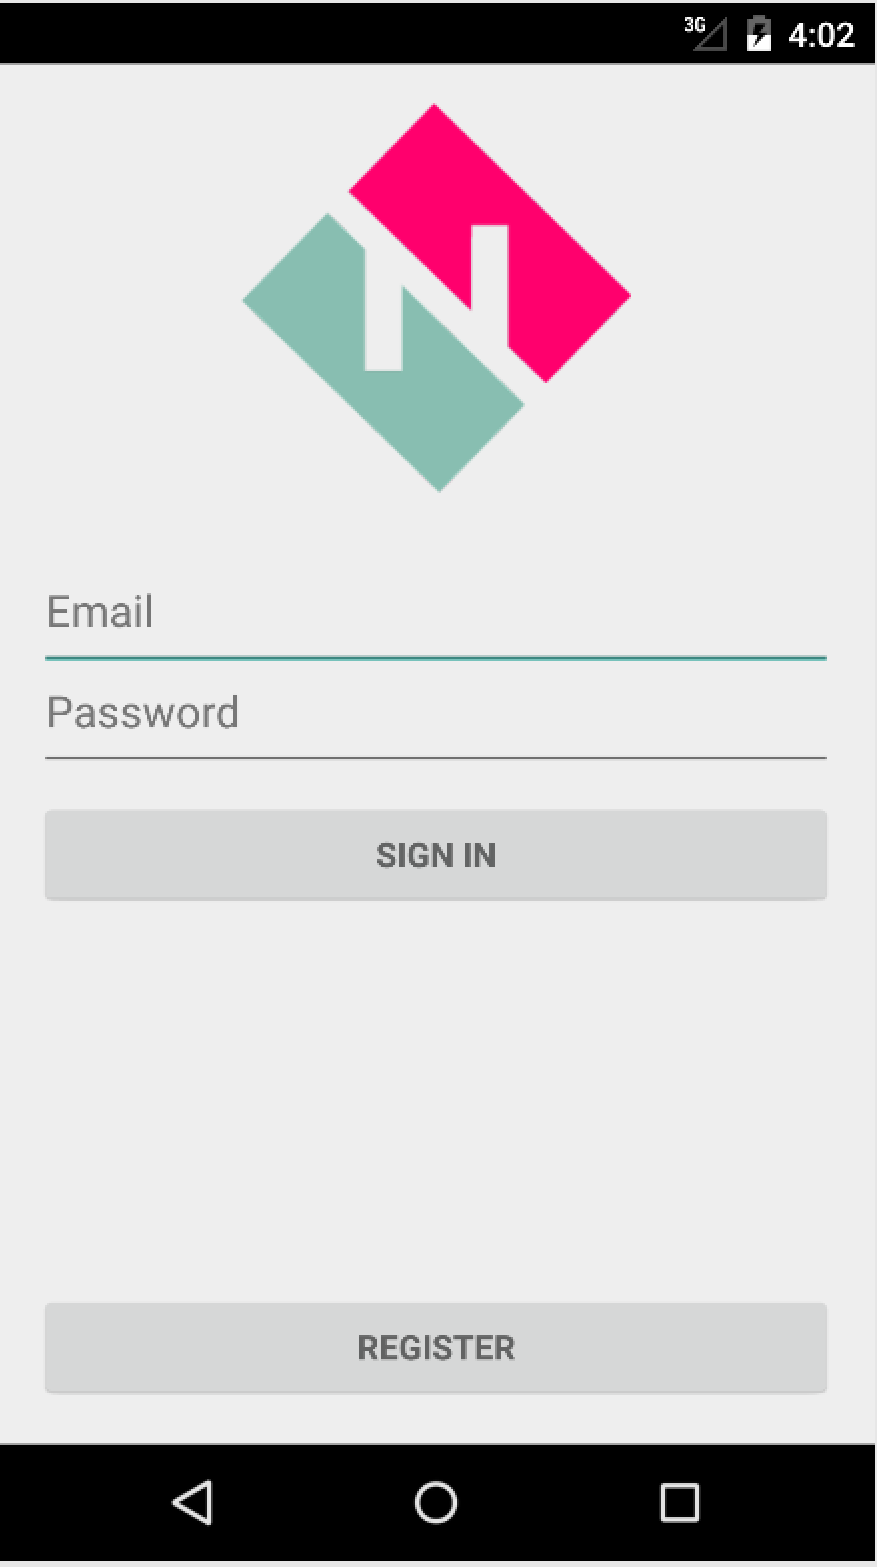
\includegraphics[width=0.9\linewidth]{./Bilder/logIn.png} 
\caption{LogIn Screen}
\label{fig:login}
\end{subfigure}
\begin{subfigure}{0.5\textwidth}
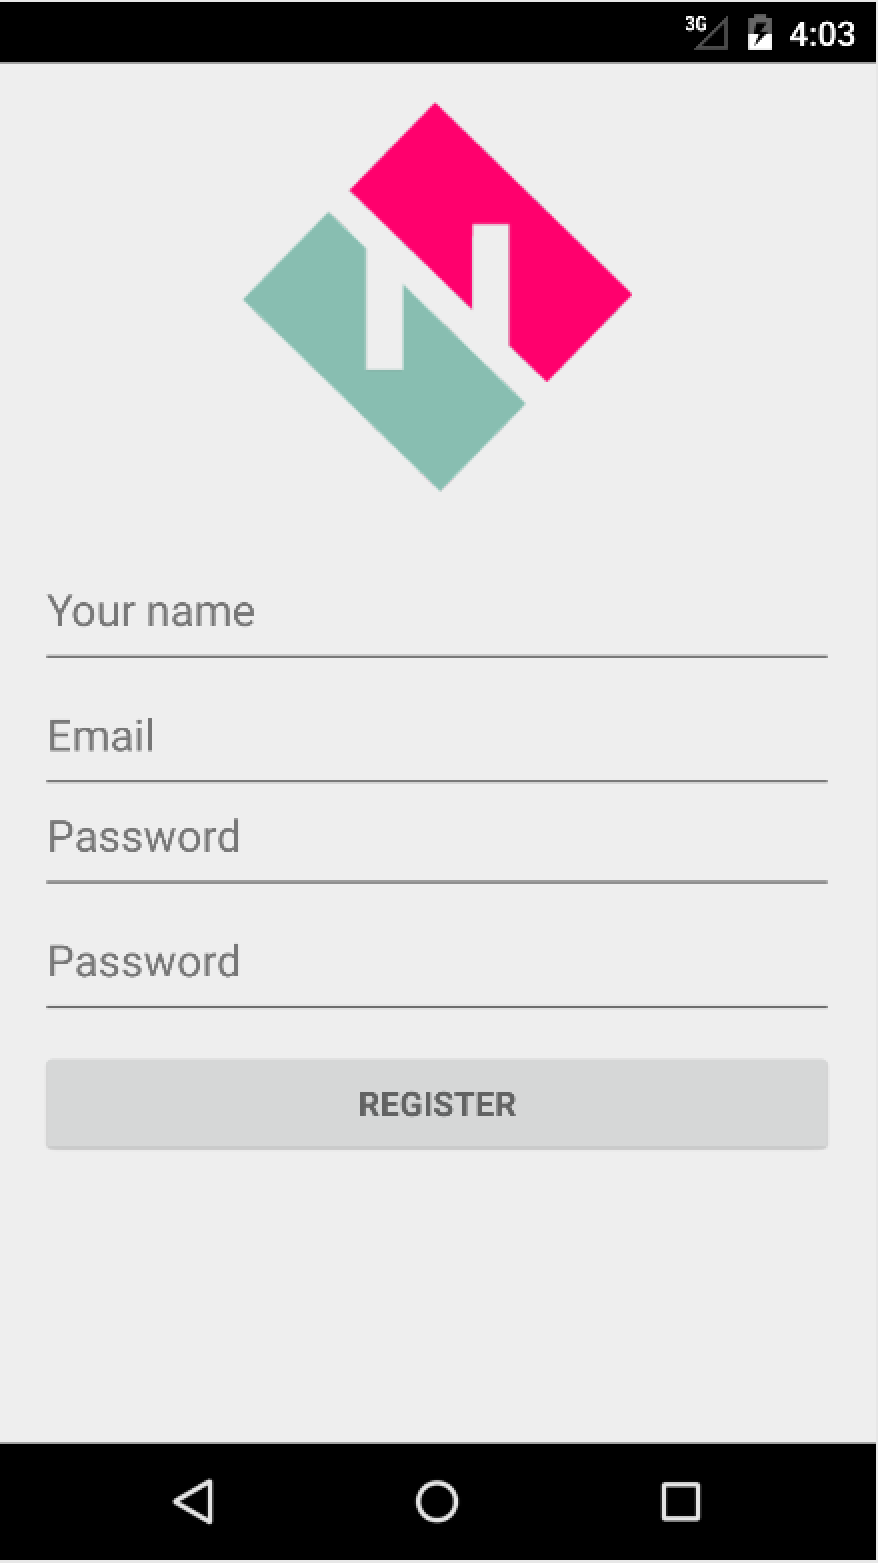
\includegraphics[width=0.9\linewidth]{./Bilder/signUp.png}
\caption{SignUp Screen}
\label{fig:signin}
\end{subfigure}
\caption{}
\label{fig:image2}
\end{figure}

Startet man die App findet man sich zuerst auf einem LogIn/SignUp - Screen wieder. 
Hier kann durch die Eingabe einer g"ultigen Email-adresse und eines Passworts ein Account erstellt, oder sich in einen bestehenden Account eingeloggt werden. 
Die Umsetzung ist schlicht und funktional gehalten. 
Dies kann so "ubernommen werden. 
 
Was erst im Vergleich mit den folgenden Seiten auff"allt, ist dass das Design dieser Seite nicht in das Schema der restlichen App passt. 
Aus Gr"unden der Konsistenz sollte das angepasst werden.

\subsubsection{Start}
\begin{figure}[H]
\begin{center}
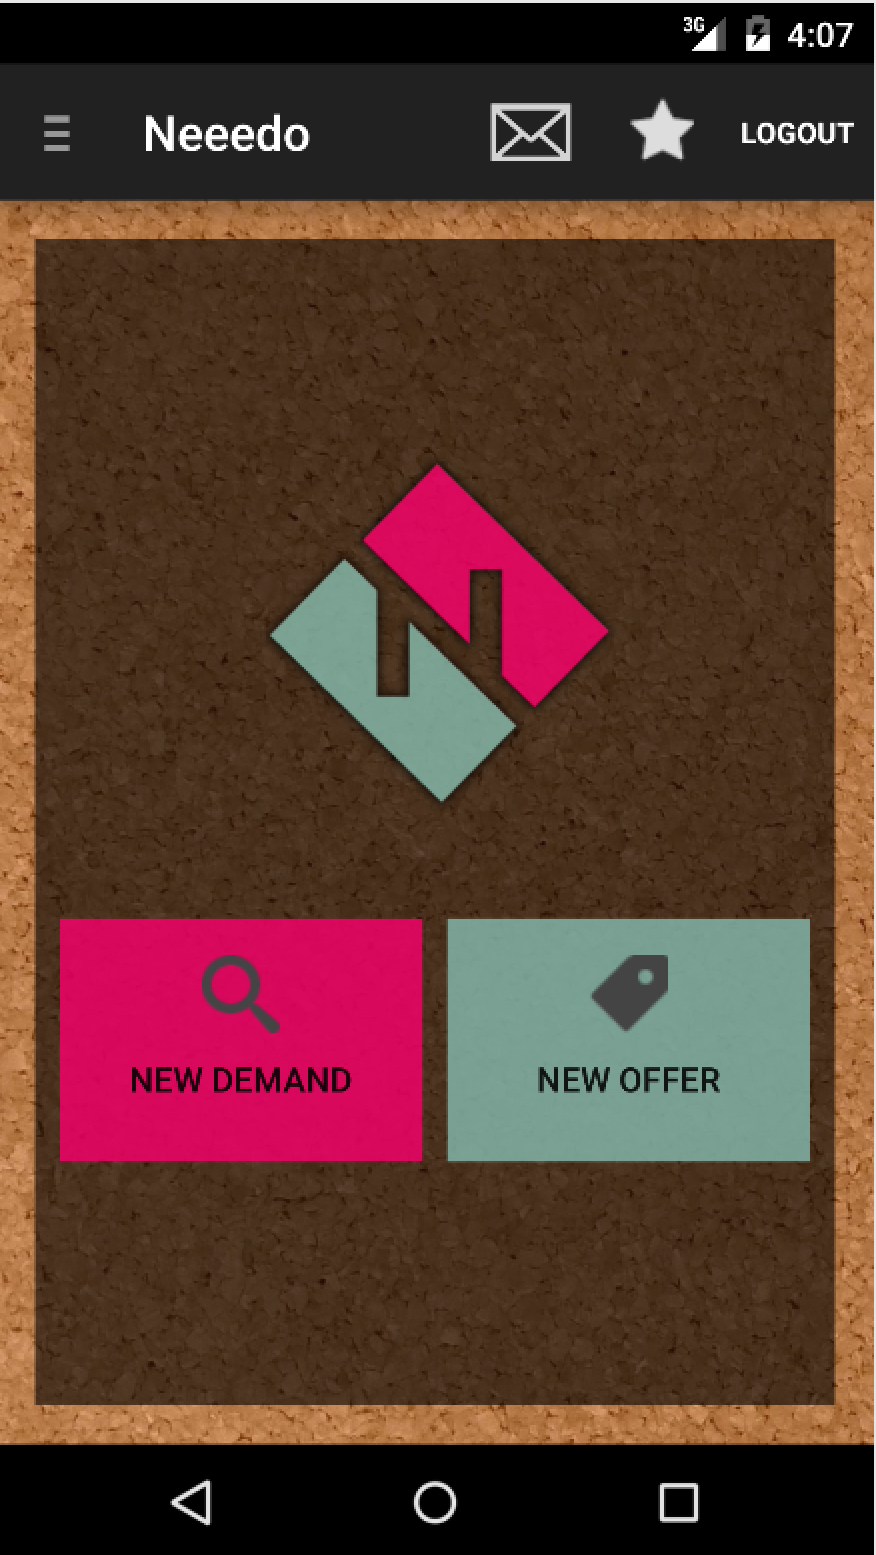
\includegraphics[width=0.45\textwidth]{./Bilder/start.png}
\caption{LandingScreen}
\label{fig:start}
\end{center}
\end{figure}

Loggt man sich in die App ein landet man zuerst auf der hier abgebildeten LandingPage. 
Diese ist schlicht gehalten.
Auf dem halbtransparenten Hintergrund finden sich zwei Button, \enquote{New Demand} und \enquote{New Offer}, die einen wohl zu den Formularen f"uhren mit denen man diese erstellen kann.
Man sieht am oberen Rand des Screens eine Men"uleiste, die einen "BurgerButton" als Men"u, den Schriftzug "Neeedo", ein Briefsymbol als Hinweis auf Nachrichten und einen Logout-Button beinhaltet. 
Dies ist eine (Android-) typische Positionierung f"ur diese  Elemente. 

Der Men"u Button ist dabei der am wenigsten markante Punkt dieses Screens, obwohl man wohl davon ausgehen kann, dass er der Wichtigste ist. 
Der Zugang zum Men"u m"usste markanter sein.

\subsubsection{Men"u}
\begin{figure}[H]
\begin{center}
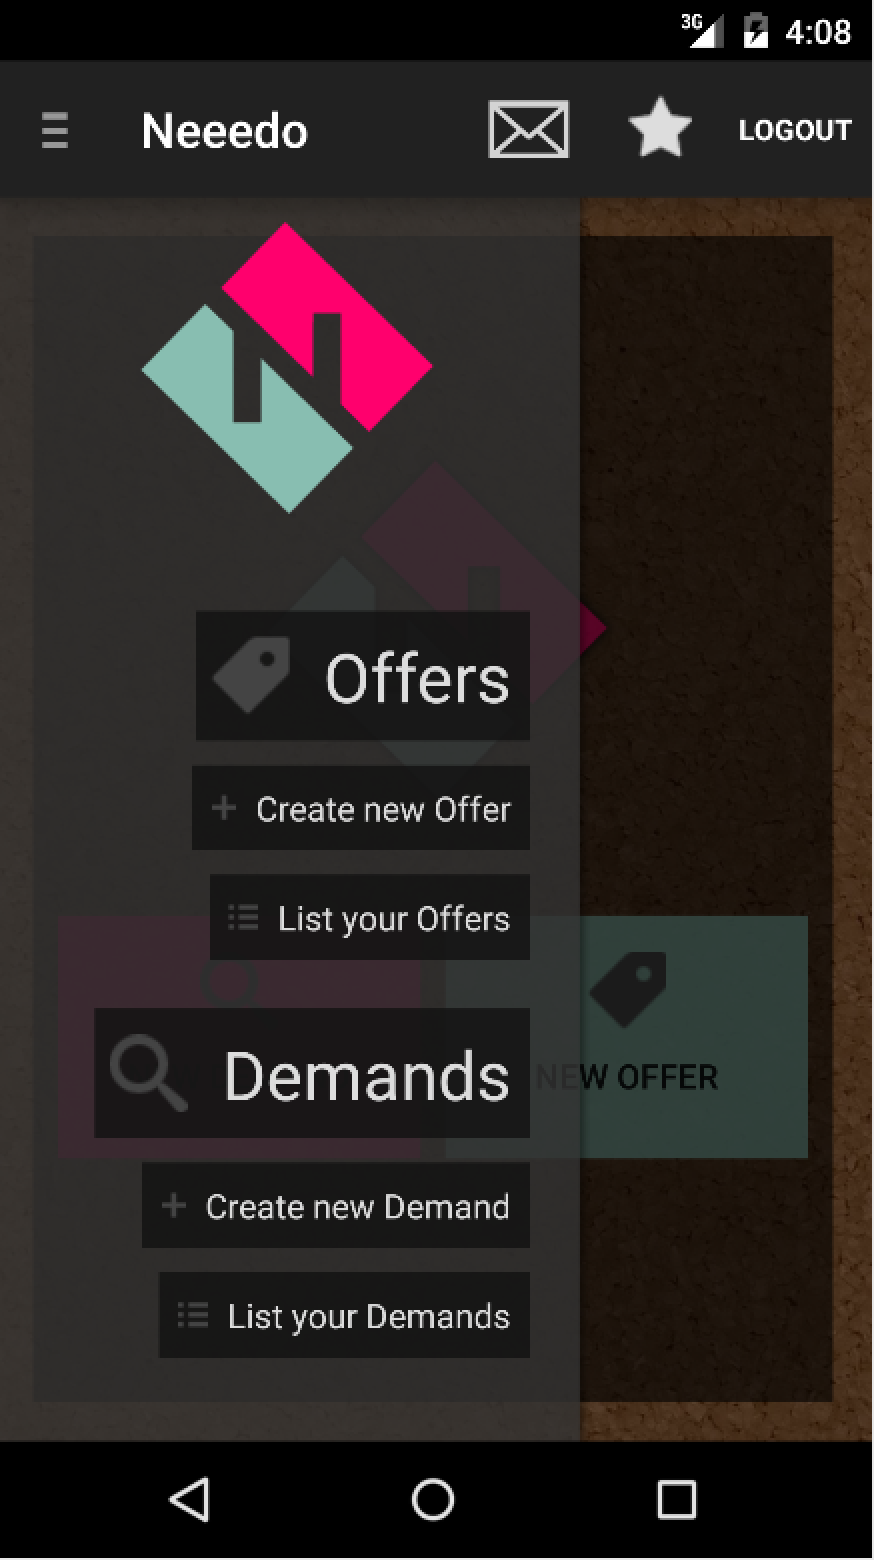
\includegraphics[width=0.45\textwidth]{./Bilder/menu.png}
\caption{Men"u offen}
\label{fig:menu}
\end{center}
\end{figure}

Benutzt man den \enquote{Men"u-Button} "offnet sich das hier abgebildete Men"u.
Dieses bietet, vier Funktionen an: \enquote{Neues Gesuch erstellen}, \enquote{Neues Angebot erstellen}, \enquote{Eigene Angebote auflisten}, \enquote{Eigene Gesuche auflisten}.

Die Umrandung um die Worte, hier, \enquote{Offers} und \enquote{Demands} l"asst vermuten, dass es sich hierbei ebenfalls um Buttons handelt. 
Dies ist jedoch nicht der Fall. 
Es handelt sich hierbei lediglich um Trenner, die das Men"u in drei Sektionen unterteilen.

Betrachtet man sich das Men"u als Ganzes f"allt auf, dass es viel zu viel Platz einnimmt und unn"otig zu sein scheint. 
Um ein solches Men"u zu rechtfertigen m"ssten mehr Funktionen angeboten werden. 

\subsubsection{Agebote und Gesuche erstellen }
\begin{figure}[H]
\begin{subfigure}{0.5\textwidth}
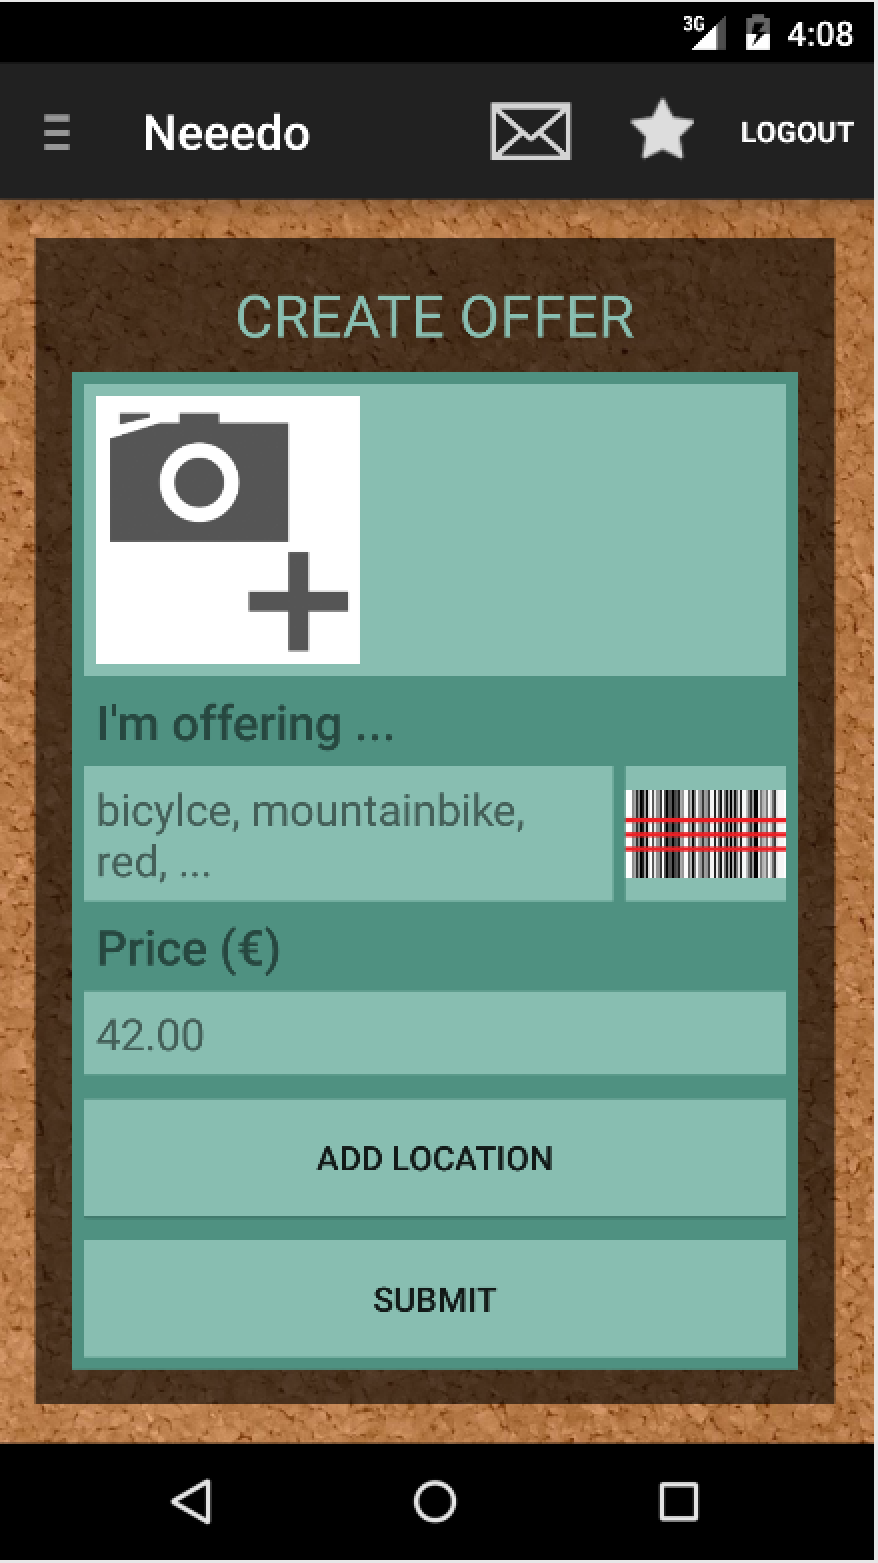
\includegraphics[width=0.9\linewidth]{./Bilder/createOffer.png} 
\caption{Angebot erstellen}
\label{fig:offer}
\end{subfigure}
\begin{subfigure}{0.5\textwidth}
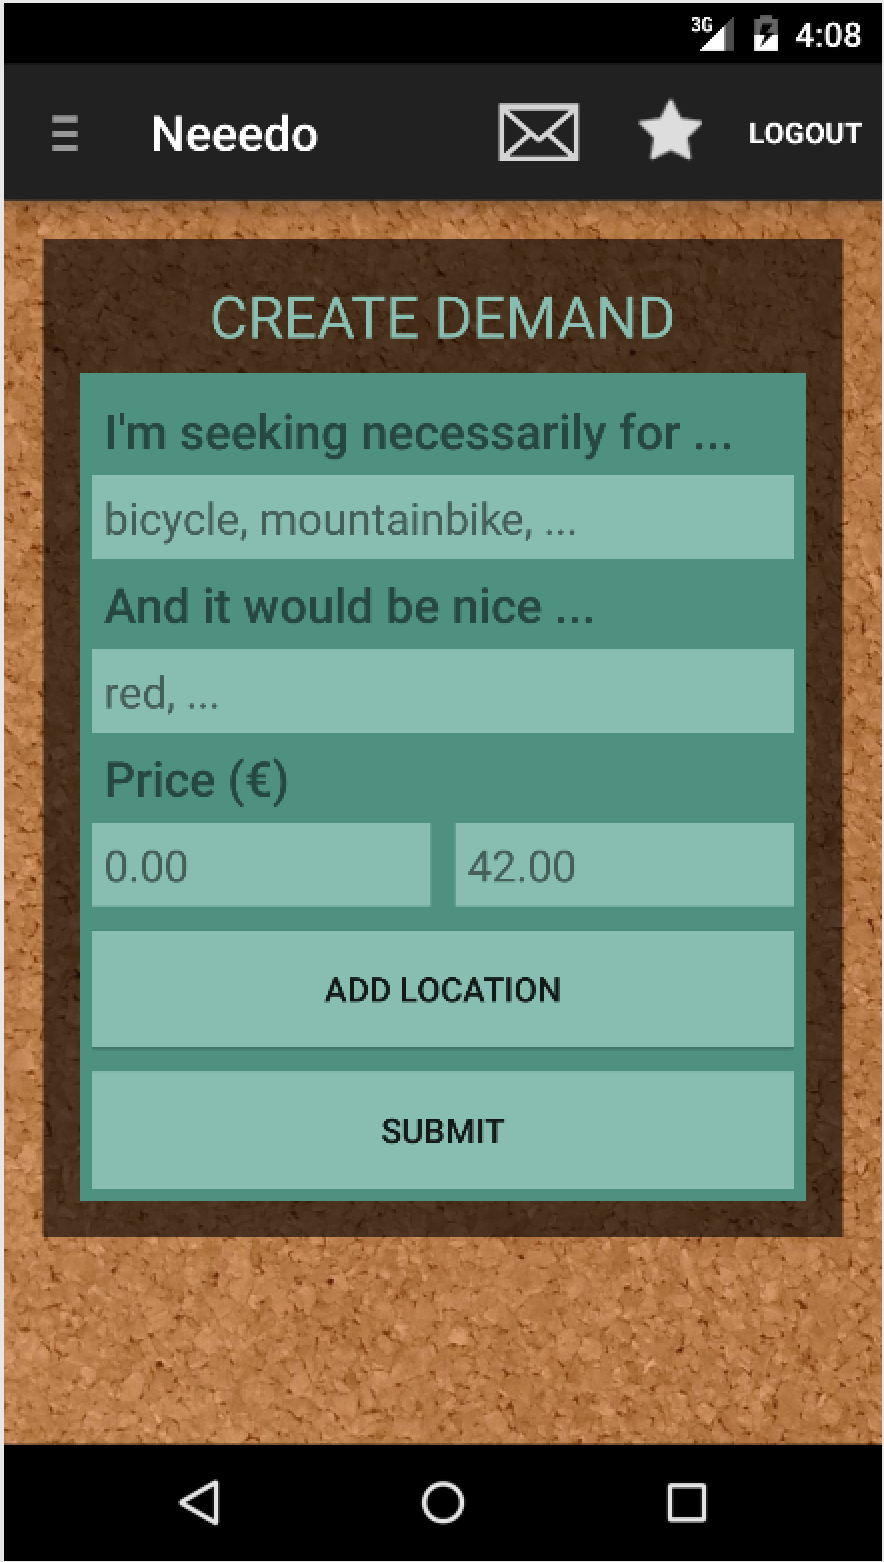
\includegraphics[width=0.9\linewidth]{./Bilder/createDemand.png}
\caption{Gesuch erstellen}
\label{fig:demand}
\end{subfigure}
\caption{}
\label{fig:image4}
\end{figure}

W"ahlt man, entweder im Men"u oder auf dem StartScreen, eine der \enquote{erstellen}-Funktionen aus, landet man auf einer dieser Seiten entsprechend der jeweiligen Auswahl.
Hier wird jeweils ein Formular angezeigt, in dem man eintragen kann was man sucht oder was man anbieten m"ochte. 

Erstellt man ein Angebot/Offer ist es m"oglich Fotos zu hinzuzuf"ugen.
Dies geschieht entweder die Auswahl des Camera-Bildes. 
Dieses ist auf den ersten Blick nicht als Button erkennbar. Dies sollte klarer erkennbar sein. 
Ebenfalls erh"allt man die M"oglichkeit informationen "uber sein Produkt durch das Scannen eines Barcodes zu erhalten. 
Diese Funktionen sind sinnvoll und k"onnten in "ahnlicher Weise "ubernommen werden.

Erstellt man ein Gesuch/Demand, bieter die App keine Zusatzfunktionen an. 
Hier muss das Formular von Hand ausgef"ullt werden.

Beide Formulare besitzen die M"oglichkeit eine Adresse hinzuzuf"ugen, dies geschieht auf einer zus"atzlichen Seite auf der dies durch Auswahl einer Positon auf einer Karte oder ein Suchfeld geschieht.

Befindet man sich auf der Formular-Seite kann man nicht klar erkennen ob man eine Position eingeben muss oder ob es einen Standardwert gibt. 
Dies sollte erkennbar gemacht werden.
 
\subsubsection{Matching}
\begin{figure}[H]
 
\begin{subfigure}{0.5\textwidth}
\includegraphics[width=0.9\linewidth]{./Bilder/matching1.png} 
\caption{Angebot erstellen}
\label{fig:match1}
\end{subfigure}
\begin{subfigure}{0.5\textwidth}
\includegraphics[width=0.9\linewidth]{./Bilder/matching2.png}
\caption{Gesuch erstellen}
\label{fig:match2}
\end{subfigure}
\caption{}
\label{fig:image5}
\end{figure}

Sendet man das auf der \enquote{Gesuch erstellen}-Seite ausgef"ullte Formular ab wird man auf die hier gezeigte \enquote{Matching-View} weitergeleitet. 
Hier werden einem passende Angebote in einer, u.a. aus der App "Tinder" bekannten Stapel-Darstellung pr"sentiert. 
Diese k"onnen entweder durch die Buttons oder durch eine Swipe-Geste nach rechts oder Links verworfen oder als Favorit gespeichert werden. 

Um die gespeicherten Favoriten aufzurufen muss man das Stern-Symbol in der Men"uleiste oben nutzen, im Screen selbst ist keine Weiterleitung m"oglich. 

\subsubsection{\enquote{Eigene} anzeigen}

\begin{figure}[H]
\begin{center}
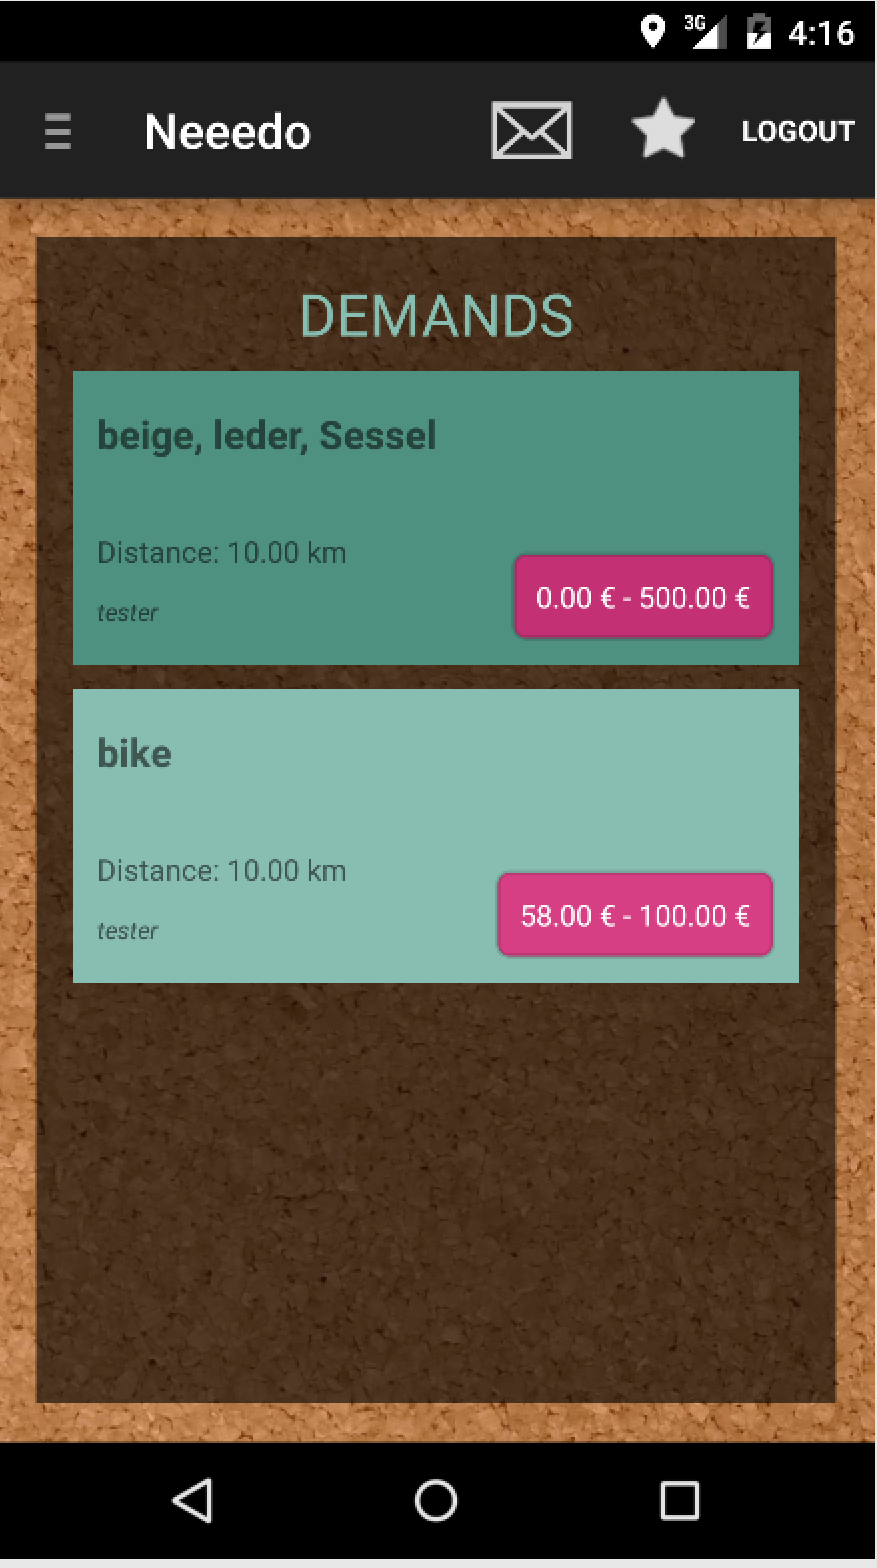
\includegraphics[width=0.45\textwidth]{./Bilder/liste.png}
\caption{Eigene Demands anzeigen}
\label{fig:anzeigen}
\end{center}
\end{figure}

Im Men"u finden sich auch die Funktionen \enquote{eigene Angebote/Gesuche anzeigen}. 
Benutzt man einen dieser Buttons, wird eine Tabelle wie die hier abgebildete pr"asentiert.
Klickt man hier auf eines der aufgef"uhrten Elemente, wird man auf ein Formular "ahnlich dem des \enquote{Erstellens} geleitet, auf dem "Anderungen durchgef"uhrt werden k"onnen. 

\subsection{Fazit}

Dies sind die wichtigsten Funktionen dieser App, weitere wie zum Beispiel der Versand von Nachrichten werden nicht n"aher betrachtet, da hier nur ein Standard Chat zum Einsatz kommt. 

\subsubsection{Positiv}\begin{description}
\item[+] Das Design ist einheitlich 
\item[+] Viele Funktionen k"onnen "ubernommen werden
\end{description}

\subsubsection{Negativ}\begin{description}
\item[-] Nicht alle Buttons k"onnen als solche erkannt werden
\item[-] Elemente k"onnen irrt"umlich f"ur Buttons gehalten werden.
\item[-] Seitenmen"u zu gro"s und unpraktisch 
\item[-] Login nicht im selben Design
\end{description}


\section{Usability-Konzept}

Basieren auf den Ergebnissen der IST-Analyse kann ein Konzept erarbeitet werden, dass die erkannten St"arken aufgreift und versucht die erkannten Schw"achen zu verbessern.

\subsection{Vorbetrachtung}

Aus der IST-Analyse und der gegebenen API lassen sich die folgenden Funktionen, bzw. Use Cases ableiten, die in der App umgesetzt werden sollen.

\subsubsection{UseCases}

\subsubsection*{Benutzer}
\begin{itemize}
\item Benutzer anlegen \vspace{-0,2cm}
\item Benutzer l"oschen \vspace{-0,2cm}
\item Benutzer ausloggen \vspace{-0,2cm}
\end{itemize}

\subsubsection*{Angebote}
\begin{itemize}
\item Angebote erstellen \vspace{-0,2cm}
\item Angebote aktualisieren  \vspace{-0,2cm}
\item Angebote l"oschen \vspace{-0,2cm}
\item Eigene Angebote anzeigen \vspace{-0,2cm}
\end{itemize}

\subsubsection*{Gesuche}
\begin{itemize}
\item Gesuche erstellen \vspace{-0,2cm}
\item Gesuche aktualisieren \vspace{-0,2cm}
\item Gesuche l"oschen \vspace{-0,2cm}
\item Eigene Gesuche anzeigen \vspace{-0,2cm}
\end{itemize}

\subsubsection*{Favoriten}
\begin{itemize}
\item Favoriten hinzuf"ugen \vspace{-0,2cm}
\item Favoriten entfernen \vspace{-0,2cm}
\item Favoriten anzeigen \vspace{-0,2cm}
\end{itemize}

\subsubsection*{Matching}
\begin{itemize}
\item Zeige passende Angebote \vspace{-0,2cm}
\end{itemize}

\subsubsection{Wie sollen diese umgesetzt werden.}

\subsubsection*{Benutzer}

Wie in der IST- Analyse bereits erw"ahnt, ist der UseCase des Nutzer-Anlegens, bzw. des User Logins bereits in einer praktikablen Weise umgesetzt.
Diese soll auch in der hier entstehenden App "ubernommen werden. 

Das Ausloggen ist in der Android Applikation durch einen Button in der Men"uleiste oben umgesetzt, jedoch besteht keine M"oglichkeit seinen Account zu l"oschen. 

In der geplanten App sollen diese beiden Funktionen zusammen in einem Men"u angeboten werden. 

\subsubsection*{Angebote, Gesuche erstellen/bearbeiten/l"oschen}

Grunds"atzlich l"asst sich an der Umsetzung des Erstellens und Aktualisierens der Angebote und Gesuche nicht viel aussetzen, au"ser einzelner Designfehler. 
Die Umsetzung mit Formularen l"asst sich nur schwer umgehen und w"urde kaum Vorteile bieten. 

Allerdings sind diese Formulare im aktuellen Zustand nicht besonders gut strukturiert und m"ussen angepasst werden, um Uneindeutigkeiten zu umgehen. 

Das L"oschen der Elemente geschieht durch einen Button auf jeweiligen Ansicht.
Dies l"asst sich ebenfalls aufgreifen. 

In iOS haben sich inzwischen aber auch, gerade in Tabellendarstellungen, Alternative M"oglichkeiten entwickelt. 
Diese sollen hier ebenfalls zum Einsatz kommen. 

\subsubsection*{Favoriten}

Das Hinzuf"ugen von Favoriten kann nur aus der jeweiligen Offer Darstellung geschehen.  Daran l"asst sich nichts "andern, da die API aktuell nur Anfgebote als Favorit zul"asst. 
In der aktuellen Umsetzung geschieht das durch einen \enquote{Stern}-Button auf der jeweiligen Karte. 

Der Stern ist eine bekannte Art der Darstellung f"ur Markierungen und Favoriten. 
Dies kann so "ubernommen werden. 

\subsubsection*{Favoriten, (Eigene) Angebote, (Eigene) Gesuche anzeigen}

Um eine "Ubersicht seiner eigenen Favoriten, Angebote und Gesuche darzustellen wurde in der Android Applikation eine Listen-Darstellung gew"ahlt. 
Diese zeigt sich als funktional und sinnvoll. 

Die Detail-Darstellung der einzelnen Elemente geschieht durch eine Karten-Darstellung auf der alle relevanten Informationen angezeigt werden.
Die grunds"atzliche Art der Darstellung dieser Elemente ist passend.
In dieser Arbeit sollen lediglich "Anderungen an inneren Struktur der Elemente durchgef"uhrt werden.

Im Rahmen der "Anderungen an der M"en"f"uhrung wird sich der Zugang zu diesen Ansichten "andern.

\subsubsection*{Matching}

In der Android Applikation werden die gematchten Angebote in der Tinder-"ahnlichen Stapeldarstellung dargestellt. 
Diese Darstellung entwickelt aktuell eine gewisse Beliebtheit und wird auch in vielen anderen Apps angeboten.
Es l"asst sich auch kein grundlegender Fehler hieran erkennen daher kann sie in einer angepassten Weise "ubernommen werden.

\subsubsection*{Men"u}

Eine gro"se Schw"ache der Android Applikation war das viel zu gro"se Seitenmen"u, dass keinen besonderen Zweck erf"ullt. 
Da die angebotenen Funktionen hier sehr begrenzt sin bietet es sich an dieses durch eine TabBar zu ersetzen. 
Diese hat den Vorteil, dass die Funktionen immer pr"asent sind und keinen zus"atzlichen Platz ben"otigen


% ----------------------------------------------------------------------------------------------------------
% Umsetzung
% ----------------------------------------------------------------------------------------------------------
\section{Umsetzung}

Die App wurde in in XCode 7.2 f"ur iOS9 entwickelt. Zur Umsetzung wurde Swift2 verwendet.  

\subsection{Vorraussetzungen}

Um diese App umsetzen zu k"onnen, mussten zuerst einige Vorraussetzungen erf"ullt werden.

\subsubsection*{API}

Damit diese App realisiert werden konnte musste zuerst eine Verbindung zur API hergestellt werden. 
Diese kommuniziert "uber RESTful Services und ist zu gro"sen Teilen nur "uber eine HTTPS-Verbindung erreichbar. 

Die API kann auf GitHub unter \url{https://github.com/neeedo/neeedo-api} bezogen werden. 
Im Normalfall bietet diese f"ur die lokale Entwicklung eine voll funktionsf"ahige Scala-Applikation die einfach "uber \textit{./sbt
run -Dhttps.port=9443} in einer Konsole gestartet werden kann. Diese ist dann unter \textit{https://localhost:9443/} 

Da Apple in der iOS-Entwicklung nur noch HTTPS-Verbindungen zu zertifizierten Diensten erlaubt, trat hier bereits das erste Problem bei der Umsetzung auf. 
Wenn die API innerhalb der lokalen Entwicklungsumgebung auf \textit{loacalhost} betrieben wird, ist aufgrund von \enquote{Server Trust problems} keine Kommunikation m"oglich.
Dieses Problem lies sich weder durch die Installation eines Zertifikats, noch den Eintrag \enquote{Allow Arbitrary Loads} in der Projektkonfiguration. beheben.

Die L"osung, die am Ende zum Erfolg f"uhrte, war die Installation der API in einem DigitalOcean-Container. Hier war es m"oglich ein Zertifikat zu hinterlegen und eine stabile HTTPS-Verbindung aufzubauen, die eine Kommunikation zwischen API und App erlaubt.

Aktuell l"auft dieser Container noch im Entwicklermodus, und muss manuell gestartet werden. 

\subsubsection*{Konfiguration}

Damit die API korrekt arbeitet m"ussen in der custom-application.conf - File Credentials zu einem Sphere-Shop hinterlegt werden. 
Um bei der Entwicklung vollen Zugriff auf die erstellten Daten zu erhalten, wurde auf  \url{https://admin.sphere.io/} ein neuer Shop angelegt. 
Die n"otigen Daten k"onnen dort unter Entwickler $\rightarrow$ API-Zugriff  gefunden werden.

\subsection{Realisierung}

Bei der Realisierung der dieser App wurde gr"o"stenteils auf den Einsatz von zus"atzlichen Libraries verzichtet, da diese nicht n"otig waren. 

\subsubsection*{Networking}
Die einzige externe Library die in dieser App eingesetzt wurde, ist Alamofire. 

Dies ist eine in Swift geschriebene Networking Library, die Funktionen zur Benutzung von REST-Verbindungen anbietet.
Eine genaue Dokumentation dieser Library kann unter \url{http://cocoadocs.org/docsets/Alamofire/3.2.1/index.html} eingesehen werden.

Der Hauptgrund f"ur die Benutzung dieser Library liegt darin, dass sie den Aufwand bei der Erstellung von HTTP-Requests vereinfacht. 
Sie stellt dabei keine besonderen Zusatzfunktionen bereit, jedoch vereinfacht sie den die Nutzung sehr. (Der ben"otigte Code wird ungef"ahr gedrittelt). 
Dies ist gerade in einem Projekt dass auf sehr vielen solcher Abfragen basiert ein gro"ser Vorteil.

\subsubsection*{Aufbau und Design}

Der Grundlegende Aufbau der App entstand durch den Einsatz in Xcode implementierten Storyboards. 
Hier wurden die ben"otigten Elemente so zusammengesetzt, dass sie die gew"unschten Funktionen erlauben. 

In der aktuellen Fassung wurden das Design beinahe vollst"andig aus Standard-UI-Elemente aufgebaut.
Lediglich einige besondere Custom-Elemente wie Pins wurden zus"atzlich verwedet. 

Wenn die App "uber einen prototypische Entwicklung hinausgeht, k"onnen hier noch ausgestaltete Custom Elemente eingesetzt werden.

Ein durchg"angiges Design wie es in der Android Applikation vorkommt, wurde nicht vollst"andig realisiert, da dies den zeitlichen Rahmen dieser Arbeit gesprengt h"atte. 

\subsection{Wie wurden die Use Cases umgesetzt?}

\subsubsection*{Benutzer}

\begin{figure}[H]
\begin{center}
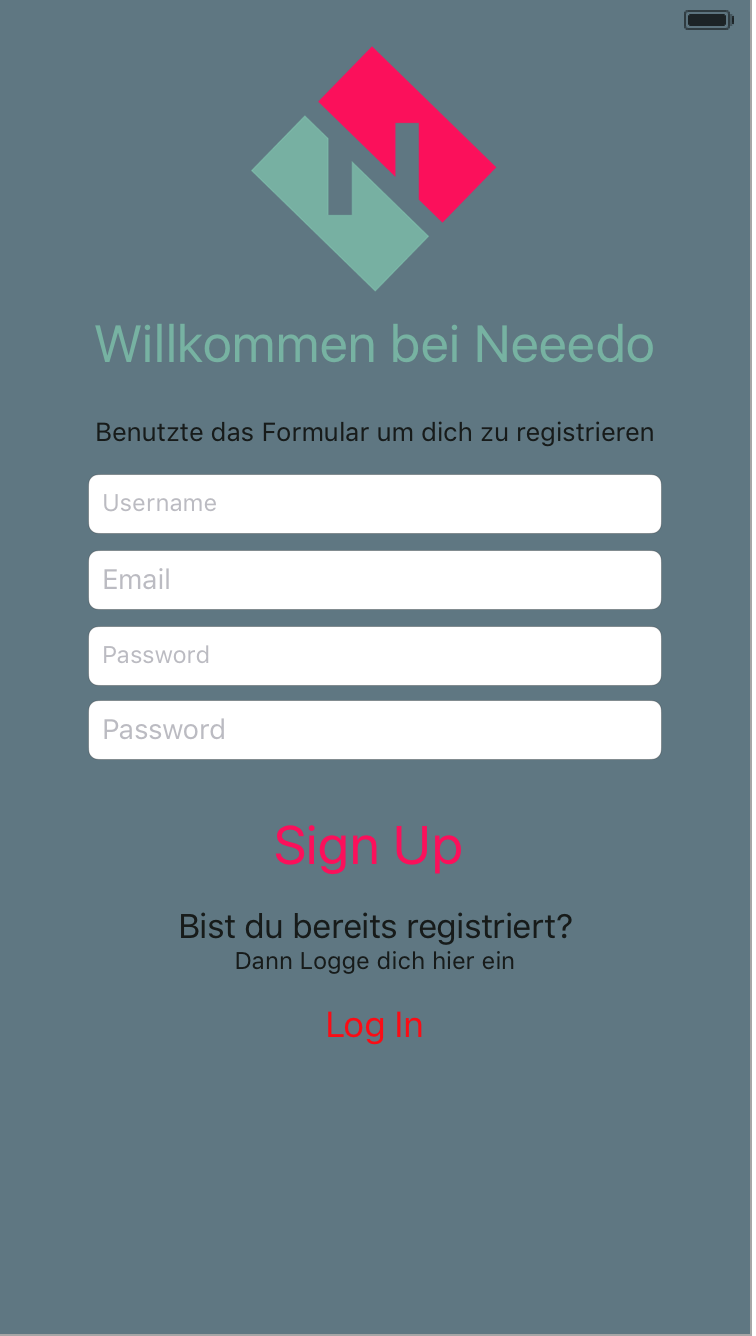
\includegraphics[width=0.45\textwidth]{./Bilder/ioslogin.png}
\caption{SignUpScreen}
\label{fig:ioslogin}
\end{center}
\end{figure}

Wie im Konzept bereits erw"ahnt wurde an der grundlegenden Struktur des Login/SignUps nichts ver"andert. Lediglich farblich wurde es an den rest der Applikation angepasst

\subsubsection{LandingScreen} 

\begin{figure}[H]
\begin{center}
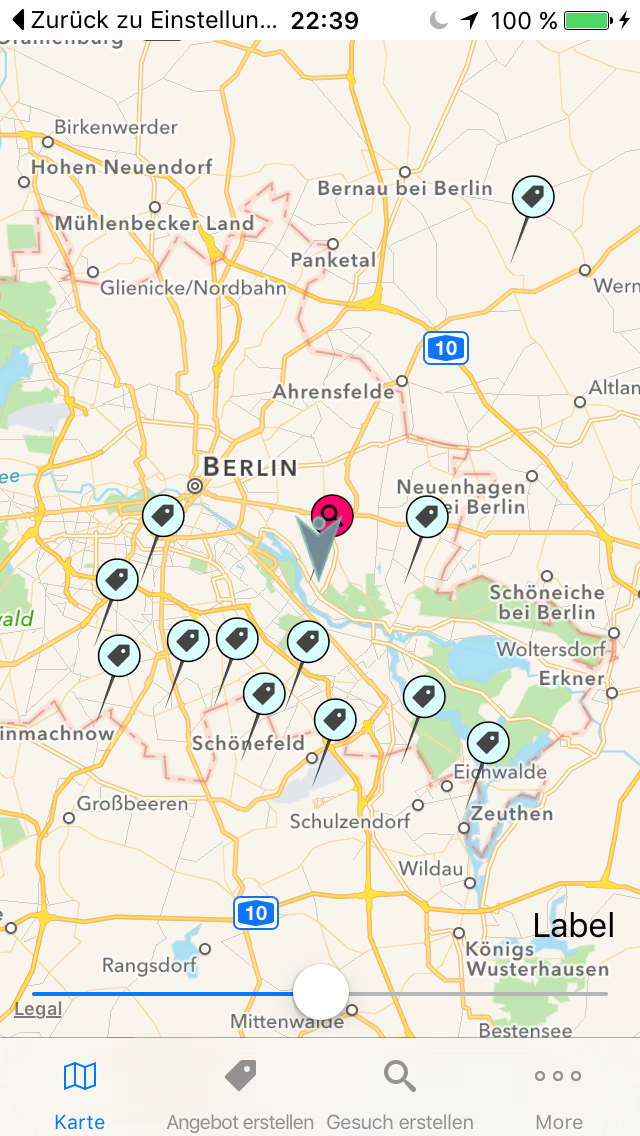
\includegraphics[width=0.45\textwidth]{./Bilder/startscreen.png}
\caption{SignUpScreen}
\label{fig:ioslogin}
\end{center}
\end{figure}

Die gr"o"ste Ver"anderung zur Android App wurde direkt auf dem LandingScreen umgesetzt. Zuvor wurden hier nur zwei  Buttons angezeigt. 
In der neugestalteten Fassung startet man auf einer Karte auf der einem direkt Angebote im Umkreis angezeigt werden. 
Diese Idee wurde so bereits in der WebApp umgesetzt. 

\subsubsection*{Men"u}

\begin{figure}[H]
\begin{center}

\includegraphics[width=0.45\textwidth]{./Bilder/tabmenu.png}
\caption{SignUpScreen}
\label{fig:ioslogin}
\end{center}
\end{figure}

Diese Ver"anderung des LandingScreens war m"oglich, da man durch die Verlagerung des Men"us in eine Tabbar keinen Bedarf mehr f"ur die beiden zentralen Buttons hatte. 
Das neue Tabbar-Men"u bietet direkten und globalen Zugang zu den wichtigen Erstell-Funktionen, "Uber den Button "Mehr" k"onnen Account spezifische Funktionen wie LogOut, Nachrichten etc. erreicht werden.

\subsubsection*{Angebote, Gesuche erstellen/bearbeiten}

\begin{figure}[H]
\begin{subfigure}{0.5\textwidth}
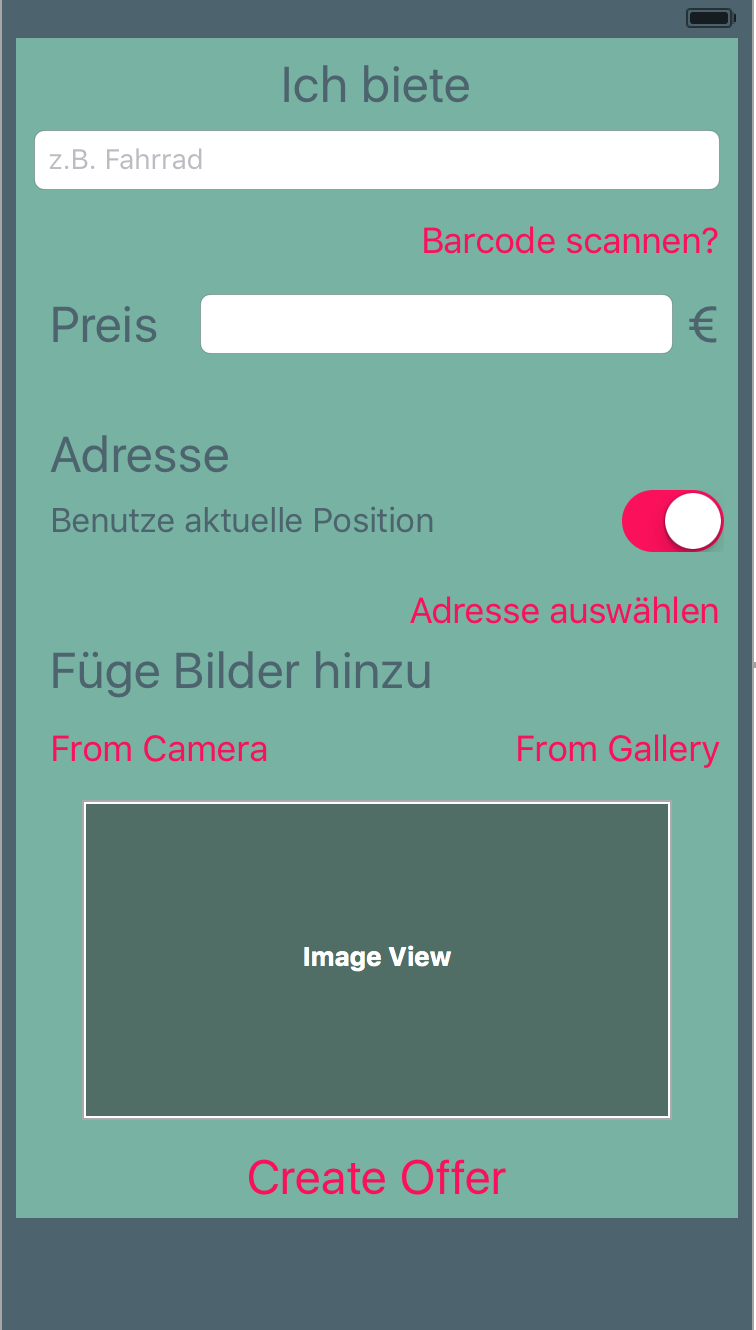
\includegraphics[width=0.9\linewidth]{./Bilder/ioscreateoffer.png} 
\caption{Angebot erstellen}
\label{fig:iosoffer}
\end{subfigure}
\begin{subfigure}{0.5\textwidth}
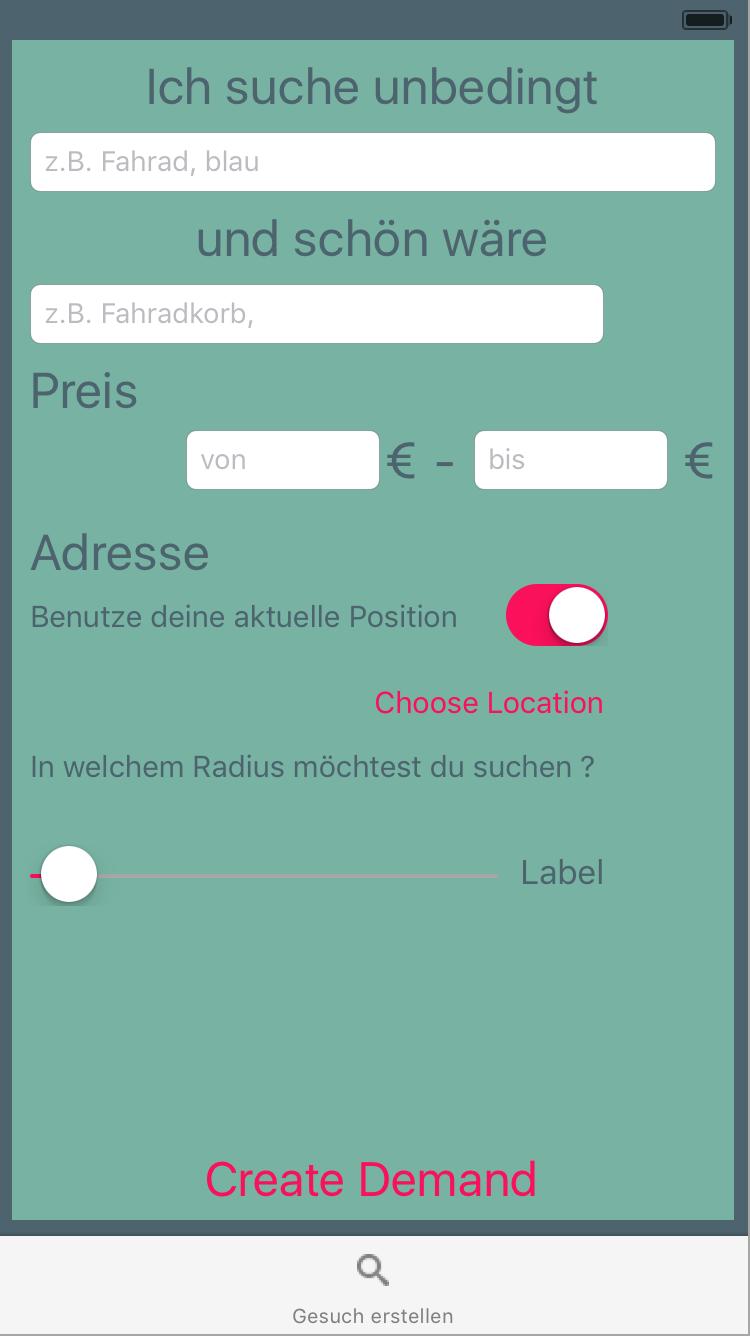
\includegraphics[width=0.9\linewidth]{./Bilder/ioscreatedemand.png}
\caption{Gesuch erstellen}
\label{fig:iosdemand}
\end{subfigure}
\caption{}
\label{fig:image10}
\end{figure}
\subsubsection*{Favoriten}

F"ur das Erstellen und bearbeiten der der Angebote und Gesuche wurde das Konzept der Formulare aus der Android Applikation "ubernommen.
Der gr"o"ste unterschied zur vorherigen Fassung ist das die auswahl der Adresse nicht mehr standardm"a"sig aktiv ist. 
Hier wurde die M"oglichkeit geschaffen direkt zu w"ahlen ob die aktuelle Position genutzt werden soll oder ob man eine andere w"ahlen m"ochte.

Im Formular zum Erstellen eines Angebotes wurden die Funktionen des Barcodescanners, sowie das Hinzuf"ugen von Bildern "ubernommen. 
Der Barcodescanner wurde dabei durch in der AVFoundation-Library zug"angliche Funktionen umgestetzt. 
Die Informationen zu den Codes werden "uber die outpan-API bzogen, die auch in der Android Applikation zum Einsatz kommt. 

Das Hinzuf"ugen von Bildern ist getrennt durch 2 Button dargestellt, um zu verdeutlichen, dass sowohl aus der Gallerie als auch von der Kamera Bilder bezogen werden k"onnen.

\subsubsection*{Matching}

\begin{figure}[H]
\begin{center}
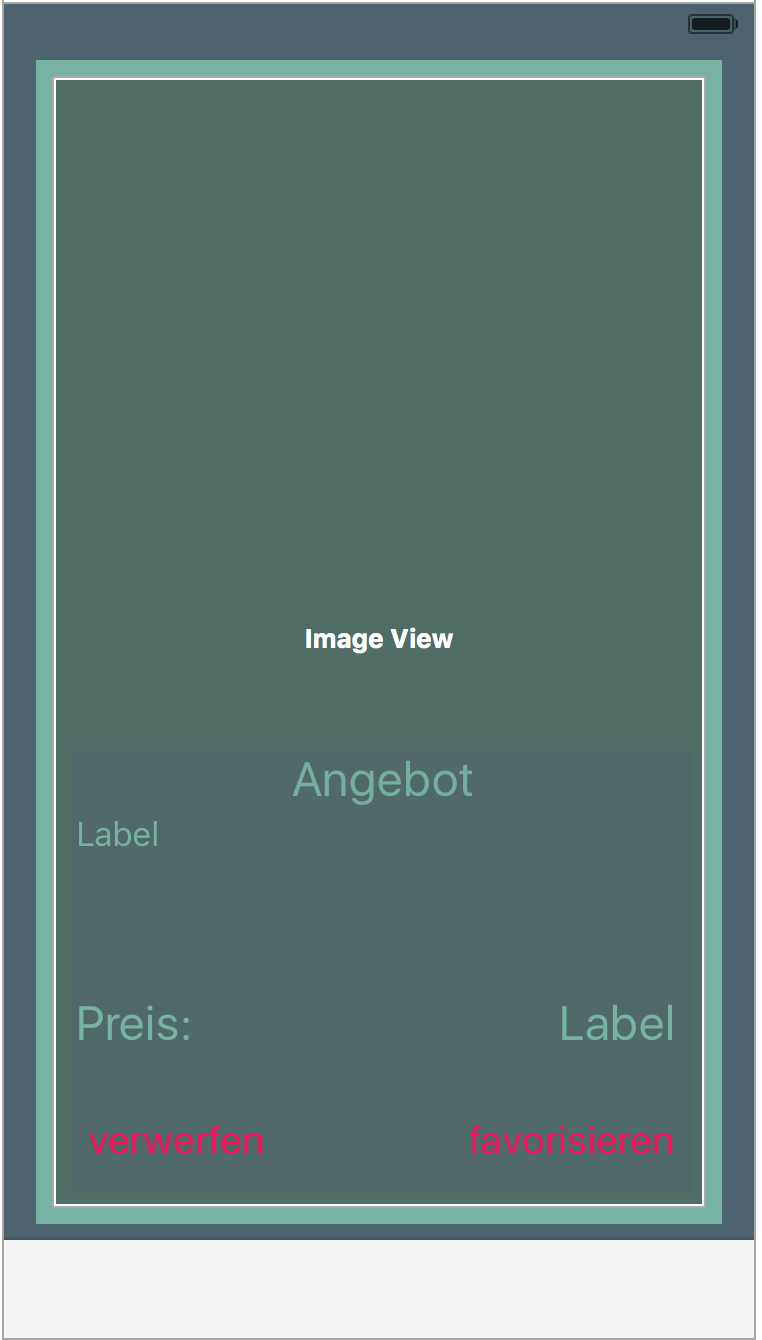
\includegraphics[width=0.45\textwidth]{./Bilder/iosmatch.png}
\caption{SignUpScreen}
\label{fig:ioslogin}
\end{center}
\end{figure}

Das Matching wurde auf ebenfalls durch die Tinder-"ahnliche Swipe ansicht realisiert. Was das Bild hier nicht anzeigt ist, dass das Angebotsbild im Hintergrund angezigt wird, und man die erwarteten Swipe-Gesten nutzen kann. 

\subsubsection*{Favoriten, (Eigene) Angebote, (Eigene) Gesuche anzeigen}

\begin{figure}[H]
\begin{center}
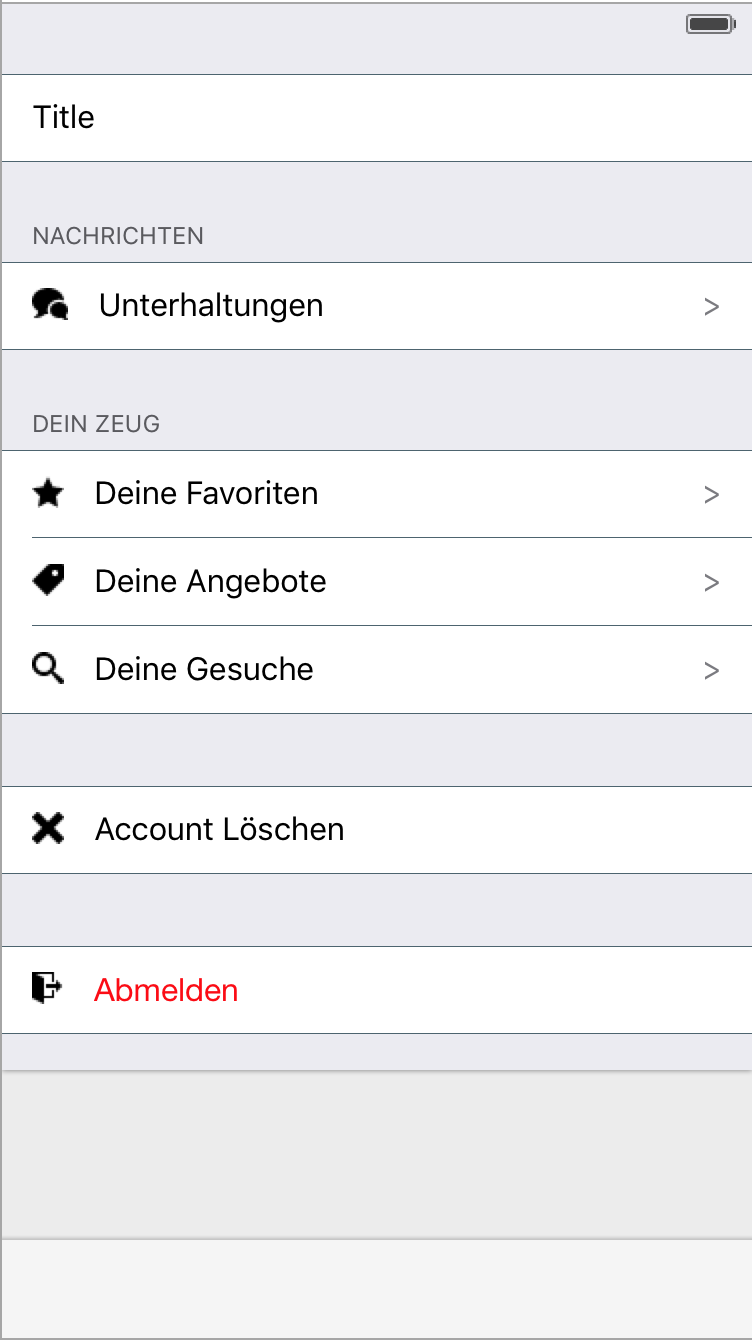
\includegraphics[width=0.45\textwidth]{./Bilder/iosMenu.png}
\caption{SignUpScreen}
\label{fig:ioslogin}
\end{center}
\end{figure}

Die restlichen Funktionalit"aten, die zuvor "uber das Kopf- oder Seitenmen"u  erreichbar waren, wurden zusammengefasst und unter dem Men"upunkt \enquote{Mehr} zug"anglich gemacht.
Hier kann man sich jetzt seine Favoriten, Gesuche und Angebote und Nachrichten anzeigen lassen. Zus"atzlich kann man hier auch seinen Account l"oschen und sich ausloggen.

\subsection{Probleme und L"osungen}

W"ahrend er Entwicklung dieser Applikation traten einige Probleme auf, diese sollen hier einmal mit ihren L"osungen dargestellt werden. 

\subsubsection{Asynchronous Programming}

Ein Problem das bei der Verwendung von RESTful Services h"aufig auftritt, ist das die Antworten(Responses) auf die Anfragen(Requests) oft eine gewisse Zeit in Anspruch nehmen. Damit die App nicht blockiert w"ahrend auf diese Antworten gewartet wird sind die Funktionen die diese Anfragen bearbeiten asynchron aufgebaut. Dies ist so sowohl in Alamofire als auch im klassischen Swift realisiert. 

Anfangs wurde dieser Fakt nicht beachtet, was zu einigen Problemen und Appabst"urzen f"uhrte. 

Die L"osung die hierbei zu verwenden ist, sind sogenannte \textit{Completionhandler} die es erm"oglichen Funktionen abh"angig von der Antwort aufzurufen, d.h. diese werden dann ausgel"ost wenn wirklich eine Antwort vorhanden ist.  

\subsubsection{Kamera}

Das Aufnehmen von Bildern mit der Kamera warf einige Probleme auf, die auch noch nicht behoben sind. Es scheint hier einen h"aufig auftretenden Bug zu geben, der beim Zugriff auf das ungespeicherte Bild auftritt. In diesem Fall erh"alt man den Fehler \enquote{snapshotting a view that has not been rendered results in an empty snapshot. ensure your view has been rendered at least once before snapshotting or snapshot after screen updates.}
Um das zu beheben muss das Bild zwischengespeichert oder angezeigt werden, jedoch scheinen danach in irgendeiner Art Probleme bei der Weiterverarbeitung aufzutreten. 




% ----------------------------------------------------------------------------------------------------------
% Fazit
% ----------------------------------------------------------------------------------------------------------
\section{Ergebnis und Ausblick }

Im Rahmen dieses Independent Courseworks wurde versucht eine Umsetzung der Ideen des Masterprojektes neeedo.com f"ur iOS 9 unter Verwendung von Swift2 zu erreichen. 
Dies sollte auf Grundlage der existierenden Android Applikation geschehen, die zuvor nach Kriterien der Usability analysiert und Umgestaltet wurde. 

Bis zum Ende des Projektzeitraumes war es m"oglich eine prototypische Umsetzung der iOS-Applikation zu erreichen, in der ein Gro"steil der angestrebten Funktionalit"aten implementiert werden konnte.

Das Projekt kann in seinem aktuellen Stand unter \url{https://github.com/Cneubauern/neeedoIOS} heruntergeladen werden.

\subsection{Ergebnis}

Die folgenden Funktionen konnten zum jetzigen Zeitpunkt umgesetzt werden.
\subsubsection*{Benutzer}
\begin{description}
\item [+]Benutzer anlegen \vspace{-0,2cm}
\item [+]Benutzer l"oschen \vspace{-0,2cm}
\item [+]Benutzer ein/ausloggen \vspace{-0,2cm}
\end{description}

\subsubsection*{Angebote}
\begin{description}
\item [+]Angebote erstellen \vspace{-0,2cm}
\item [+]Angebote aktualisieren  \vspace{-0,2cm}
\item [+]Angebote l"oschen \vspace{-0,2cm}
\item [+]Eigene Angebote anzeigen \vspace{-0,2cm}
\end{description}

\subsubsection*{Gesuche}
\begin{description}
\item [+]Gesuche erstellen \vspace{-0,2cm}
\item [+]Gesuche aktualisieren \vspace{-0,2cm}
\item [+]Gesuche l"oschen \vspace{-0,2cm}
\item [+]Eigene Gesuche anzeigen \vspace{-0,2cm}
\end{description}

\subsubsection*{Favoriten}
\begin{description}
\item [+]Favoriten hinzuf"ugen \vspace{-0,2cm}
\item [+]Favoriten entfernen \vspace{-0,2cm}
\item [+]Favoriten anzeigen \vspace{-0,2cm}
\end{description}

\subsubsection*{Favoriten}
\begin{description}
\item [+]Favoriten hinzuf"ugen \vspace{-0,2cm}
\item [+]Favoriten entfernen \vspace{-0,2cm}
\item [+]Favoriten anzeigen \vspace{-0,2cm}
\end{description}

Aktuell gibt es noch Probleme beim Matching, dieses f"uhrt unter bestimmten Umst"anden zu Abst"urzen, sowie beim ImageUpload von der Camera. 
Das Messaging System wurde als Ansicht implementiert ist aber noch nicht funktionsf"ahig 
Das von der neeedo-API angebotene Tag-Suggestion-System wurde aus zeitgr"unden nicht mehr bearbeitet. 

\subsection{Ausblick}

F"ur die Zukunft gilt es vor allem an der Konsistenz und am Design zu arbeiten. Es sind noch viele kleine und Mittelgro"se Bugs zu beheben und die beschriebenen Funktionalit"aten vollst"andig umzusetzen. 

\subsection{Res"umee}

F"ur mich war dieses Projekt eine interessante Herausforderungen. Zwar habe ich in der Vergangenheit bereits Erfahrungen mit der iOS Entwicklung gemacht, doch war Swift2 noch sehr neu f"ur mich. 
Ebenso war dies die erste iOS-App mit Netzwerkanbindung die ich selbst entwickelt habe. 
Ich konnte im Verlauf des Projektes viel lernen und neue Erfahrungen machen. 


% ----------------------------------------------------------------------------------------------------------
% Ausblick
% ----------------------------------------------------------------------------------------------------------

\end{document}
